% -------------------------------------------------------------------------------------
\chapter{Fairness} \label{chap:fairness}
% -------------------------------------------------------------------------------------

So far, we have discussed recommender systems in general and the methods that are used in the field. However, now, let us step back and look at the problem from a broader perspective of fairness as a social construct.
Specifically, we will focus on the importance of fairness in the context of algorithms.
What role fairness plays when using machine learning models with potentially sensitive data, and if we can make group recommenders better when we understand and define fairness and its underlying properties better.

We will start with a general introduction to the topic of fairness, define its possible meanings and specify which one is important in our setting.
This is required due to the overload of the word itself and the rising importance of the topic in today's world. Furthermore, we will explain why fairness seems to be a crucial parameter in the group recommender setting and will try to reason about how to measure its effects.




% -------------------------------------------------------------------------------------
section{General} \label{sec:02_general}
% -------------------------------------------------------------------------------------

The word fairness itself is hard and controversial to define. In Cambridge Dictionary \cite{fairness_definition}, it is defined as "The quality of treating people equally or in a way that is reasonable." Its use has been rising steadily since the 1960s, as we can see in Figure \ref{fig:popularity_of_fairness}.

\begin{figure}[htbp]
    \centering
    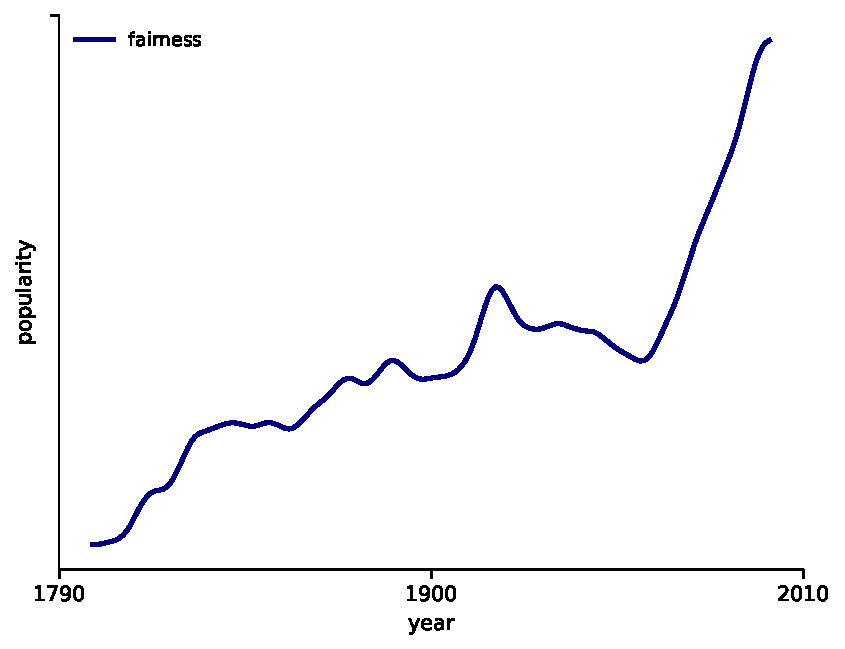
\includegraphics{img/google_ngram_fairness-eng_2012-1800-2000.pdf}
    \caption{The graph shows the phrase "fairness" occurring in the corpus of English books from 1800 to 2010. Source: Google Ngram Viewer, corpora 2012. \cite{google_ngram_viewer_2012}}
    \label{fig:popularity_of_fairness}
\end{figure}

Humans are obsessed with fairness. From a young age, children will get sad when something is not fair, when their sibling gets a more significant piece of the pie, more attention from their parent, or any other unequal situation. It can induce strong emotions such as envy, sadness, or anger, and it emerges very early, as early as 12 months of age or sooner, as researched in \cite{children_fairness}.

Furthermore, this behavior is not limited only to humans. We can observe the same behavior in monkeys. In \cite{brosnan2003monkeys}, the authors observed that if a monkey is getting the worse reward for the same task as its peer,  it refuses the reward and demands the same payout even if they were satisfied with the lesser reward for the same task before. In some sense, this is very strange; why should we care about someone having more if we have enough?

We observe the same behavior in many other species of animals, but not all. It seems that it requires a certain level of intelligence for the notion of fairness to emerge. As discussed in \cite{brosnan2014evolution}, based on studies of other non-human species, this evolutionary puzzle can be further dissected into responses to reward distribution among the cooperating group members. Humans are willing to seek an equalization of outcomes even if it means that they will lose some of their own reward as studied in \cite{willing_to_pay_to_equality}. At the same time, we humans like 'free rides' where we get high rewards for a small amount of work but dislike when someone else gets the same. This directly corresponds with fairness itself --- It is not fair if someone else gets something we do not. However, it all depends on our personality and the type of relationship involved. Some people are, for example, willing to accept that their partner makes more, but that is very subjective and sometimes can even lead to larger envy.

In some cases, we observe a pattern of generosity, where children are willing to make their own sacrifices in order to ensure fairness so that the other person does not have less than them, as presented in \cite{children_generocity_blake}. The authors studied fairness in multiple cultural settings and found that this behavior is learned and only present in some cultures.

On the other hand, our society widely accepts the notion of 'winner takes all', which can be problematic in itself, for example, in sports and business. In business, it directly shapes the distribution of wealth, which is considered one of the main problems of today's world. Nevertheless, discussing the social aspect of fairness is beyond the scope of this thesis.

Regarding the true nature of fairness on the deepest level, it could even be possible that the notion of fairness emerges together with cooperation, language, and communication. It would mean that it is an inherent property of any intelligent agent created through an evolutionary process.
Another point of view could be that fairness acts as a mechanism that pushes towards equality among the group members, leading to higher stability of the group, which would give an evolutionary advantage.

However, more research has to be done, as our understanding of intelligence, consciousness, and related hard-to-quantify phenomena are lacking.

Let us now get back to fairness in the context of computer systems.

% -------------------------------------------------------------------------------------
\section{Algorithmic fairness}\label{subsec:02_general.algorithmic_fairness_and_possible_meanings}
% -------------------------------------------------------------------------------------
%The Emerging Theory of Algorithmic Fairness

We will focus on fairness regarding society or individuals interacting with a computer system. We will not discuss further any meaning of fairness outside of the domain of computer science. This topic steers away from the primary goal of defining fairness for the group RS sub-domain, but we think that it is a very important topic in general, and therefore it deserves more spotlight and can be an excellent middle step to understanding specifics of the group RS setting.

% -------------------------------------------------------------------------------------
\subsection{Sources of algorithmic unfairness}
% -------------------------------------------------------------------------------------

How can a computer with no underlying understanding of race or ethnicity discriminate against a group of people? At first, this idea may seem strange, but we have to remember that, as with any other computer program, machine learning algorithms are designed by people. Data used to train those algorithms comes from the real world, where bias and unfairness are unfortunately still present. Thus, the trained models, even if not usually meant with an ill-fated purpose, will reflect that and, in most cases, include some form of bias or unfairness.
Of course, there exist uses of ML with bias that has been introduced on purpose. We can see that for example in the Chinese credit score system which is biased towards an individual based on their class, race, political views, and other factors. Which we, in the modern democratic world, consider as protected(sensitive) characteristics, that are not to be used to discriminate against an individual. However, this type of bias in those circumstances is a knowingly designed and required feature of the system; therefore, we will not discuss these systems any further.

More rigorously, we can say that output of any machine learning (ML) algorithm is usually just a product of the underlying data. An accurate classifier will reproduce patterns found in the training data by design. Usually, the bias is either transferred directly from the data or by wrongly defining the learning objective.

Let us now present a division by the main sources of unfairness as stated in \cite{pessach2020algorithmic_fairness} with examples following in Subsection \ref{subsec:02_algo_fairness.examples_of_algo_biass}:
\begin{itemize}
    \item \textbf{Biases already included in the dataset}\newline
    Such as dependence/correlation of data based on sensitive characteristics. An accurate classifier by design reproduces bias found in the data.
    \item \textbf{Biases caused by missing data}\newline
    Missing or filtering out some of the training data can result in a dataset that does not represent the target population.
    \item \textbf{Biases stemming from algorithmic objectives}\newline
    While training, we usually minimize some error, which can lead to a prioritization of the majority's interests if left unchecked. It will always be easier to optimize results for groups with small entropy, than for niche groups that are more surprising and thus have a larger entropy.
    \item \textbf{Biases caused by "proxy" attributes}\newline
    Some attributes that are not directly considered sensitive can still contain information from sensitive attributes. In other words, they are not independent. Therefore, the algorithm can use the "proxy" attribute and indirectly exploit the sensitive attribute.
\end{itemize}


It is important to define which sensitive characteristics need to be considered. As stated in \cite{european-union-agency-for-fundamental-rights-2018} those are gender, ethnicity, sexual orientation, disability, and others. Most research in the domain of bias and fairness is, based on our perception, studied from the perspective of discrimination and the impacts of algorithms on society. We observe bias against specific groups of the population based on their race, sex, nationality, education, beliefs, and many other attributes (protected as well as unprotected ones), which causes a measurable impact on our everyday life. After all, we are more than ever involved and surrounded by technology. Therefore, it is essential to understand the effects biased algorithms can have and to study techniques and strategies to mitigate their negative impact.


Further, we can also view fairness from the aspect of algorithmic decision-making, where a decision process can introduce unfairness based on some non-deterministic property or computation. Some sectors, such as justice and finance, have to strive for equality of outcome due to the high cost of errors of unfair decisions, either in the form of unjust punishments in the former case or financial loss in the latter.



% -------------------------------------------------------------------------------------
\subsection{Examples of algorithmic bias}\label{subsec:02_algo_fairness.examples_of_algo_biass}
% -------------------------------------------------------------------------------------
We will now present a few instances of computer systems that have been used in settings where a bias towards a sensitive characteristic had a substantial impact.


\begin{itemize}
    \item \textbf{Amazon's automatic recruiting system}\newline
    As reported by \cite{amazon-unfair-hiring-2018}, in 2018, it was found that the new system for hiring people for Amazon was biased toward women. The IT field is mostly male-dominated - women represent only around 23\% as stated in \cite{women-in-tech-2021}. Due to this disproportion, the algorithm discovered in training data pattern between the gender of the candidate and hiring results which led it to assume that male candidates are preferred before female ones. The algorithm was not told the gender of the candidate, but it inferred it from other data such as university, hobbies, and others. This bias is a combination of 'bias already included in the dataset' and 'biases caused by proxy attributes'. The company later disbanded the team and left the tool only as a helper tool that works in conjunction with the recruiters instead of solely automatically.
    
    \item \textbf{Apple's credit card}\newline
    Apple released its credit card in 2019. It works as follows: after the sign-up, the user receives a certain credit limit from the service provider (Goldman Sachs). Some people, as reported in \cite{apple-card-washingtonpost-2019}, noticed that their wives were assigned smaller credit limits even though their credit score was higher and they only had one shared bank account.
    In this case, an investigation by the New York State Department of Financial Services came to a conclusion based on an extensive analysis that no unlawful discrimination against applicants has taken place.
    
    \item \textbf{COMPAS} - Correctional Offender Management Profiling for Alternative Sanctions\newline
    COMPAS is an algorithm used in the US justice system to predict the likelihood of a defendant becoming a recidivist. Analysis \cite{compas-analysis-2020} found that black defendants were often predicted as being at higher risk than they actually were. On the contrary, white defendants were predicted to be less risky than in reality. In the case of re-offended, this predicted risk was almost twice as high for blacks compared to whites. They conclude that the tool is imprecise and does not reflect the actual likelihood it was designed to predict.
\end{itemize}

In these cases, society, and mainly the law, has to act and protect those that are treated unfairly. European law can act as an excellent example of what can be done. The general data protection regulation (GDPR) and the protection of individuals against algorithmic bias are great and functioning examples.

Details about laws that are in effect in the EU and definitions of sensitive characteristics and areas of protection can be found in Handbook on European non-discrimination law \cite{european-union-agency-for-fundamental-rights-2018}.


% -------------------------------------------------------------------------------------
\subsection{Measures of algorithmic fairness}
% -------------------------------------------------------------------------------------
We need to have a precise way of measuring bias towards sensitive characteristics to design and evaluate algorithms that are taking or should take measures to ensure fairness. 

At first sight, our idea could be to remove features that we consider sensitive entirely from the dataset, but that will, in most cases, not suffice due to other features being slightly correlated with the sensitive feature. Correlation with, for example, gender will probably be too small to be predicted with measurable accuracy. However, this balance can tip over if we combine many of these slightly correlated features. We, therefore, need to approach this problem more rigorously.

We now present a few statistical methods as mentioned in \cite{fairness_ml_book_2017}:
\begin{itemize}


    \item \textbf{Independence}
        We say that sensitive characteristic Char is independent of a prediction Pred if:
        \begin{equation}
            P\left(Pred = p|Ch = a\right)=P\left(Pred=p|Char=b\right) \quad \forall p\in Pred \quad \forall a,b \in S
        \end{equation}
        is the probability of the given prediction being the same for two people from different groups with respect to the sensitive characteristic.
    
    
    \item \textbf{Separation}
        We say that random variables $(Pred,Char,Y)$ satisfy separation if the sensitive characteristics $Ch$ are statistically independent of the target value $Y$ given the prediction $Pred$.
        This relation can be expressed with:
        \begin{equation}
        \begin{split}
            P\left(Pred=p|Y=q,Char=a\right)=P\left(Pred=p|Y=a,Char=b\right) \\
            \quad \forall p\in Pred\quad q \in Y \quad \forall a,b \in Char
        \end{split}
        \end{equation}
        Meaning that the dependence of a prediction result on the sensitive attribute $Char$ can be justified by the attribute $Char$ being dependent on $Y$.

    \item \textbf{Sufficiency}
        We say the random variables $(Pred,Char,Y)$ satisfy sufficiency if the sensitive characteristics $A$ are statistically independent of the target value $Y$ given the prediction $R$. This can be expressed as:
        \begin{equation}
        \begin{split}
            P\left(Y=q|Pred=p,Char=a\right)=P\left(Y=q|Pred=p,Char=b\right) \\
            \quad \forall q\in Y\quad p \in Pred \quad \forall a,b \in Char
        \end{split}
        \end{equation}
        We say that $Pred$ satisfies sufficiency i the target variable $Y$ and the sensitive attribute $Char$ are clear from the context.

    
\end{itemize}


% -------------------------------------------------------------------------------------
\subsection{Outcome vs. opportunity}
% -------------------------------------------------------------------------------------
From separation and sufficiency, we see that there is only a difference in the direction of the relationship between random variables $Pred$ and $Y$. We will call them 'equality of opportunity' and 'equality of outcome', respectively.

Let us now present an example of both. We have a model situation where we strive for gender equality in the management of our company.

\begin{itemize}

    \item \textbf{Equality of outcome}
    We would like the resulting distribution to be fair such as there has to be 50\% male and 50\% female gender representation among our management. If we have more than 50\% men, we need to fire them and hire only women. It may seem easy, and this is where most of the efforts usually stop, but even just finding what the desired resulting distribution needs to look like is a non-trivial task.
    \item \textbf{Equality of opportunity}
    In this case, we try to mitigate any bias that could skew the decision of whom to hire towards any gender. Preferably, we do not want to even propagate the fact about the protected attribute (in this case, gender) to the people making the final decision.
    
\end{itemize}


Both of these cases/methods have their place but should be used cautiously. They can cause a great deal of fairness equalization when used correctly but, at the same time a great deal of harm when implemented incorrectly.


With the already discussed topics in mind, we can connect the fairness and the group recommendation systems with the subsequent possible interpretation. What applies to our group recommender domain is the notion of fairness in the sense of a balance of preference between group members. Each member has their preference, and we are trying to balance them in the best possible way so that everyone likes the recommended object or list of objects equally.

Further, if we take group membership as a sensitive attribute of the group and consider it a sensitive attribute, then we want independence in the context of equality of outcome.

% -------------------------------------------------------------------------------------
\subsection{General methods of prevention}
% -------------------------------------------------------------------------------------
Thanks to machine learning models being entirely dependent on the data, as discussed previously, we can divide the general techniques of bias suppression by where the change to the machine learning process is made on the data path. We divide the general techniques into three categories as follows:
\begin{itemize}

    \item \textbf{Pre-processing}
    Adjust training data in a way that sensitive characteristics are uncorrelated. 
    
    The main benefit of preprocessing data this way is that if we ensure independence this way, then any subsequent deterministic method will transitively also satisfy the independence of the sensitive attributes.
    Nevertheless, as with any data transformation that changes data properties and distributions, we need to be careful not to hinder the efficacy of the final model.
    
    \item \textbf{At training time}
    Design algorithms that set constraints on the optimization process itself.
    
    This change seems to be the hardest to technically and algorithmically implement. We need access to the whole collection of raw data to ensure that we are not biased. Furthermore, we limit ourselves to ML methods that allow this constrain modulation. On the other hand, the main benefit is that we perform the optimization with full information of the task and, therefore, can potentially gain more utility.
    
    
    \item \textbf{Post-processing}
    Adjust parameters of the already learned classifier so as to be uncorrelated with the sensitive attribute.
    
    This is the least favorable from the theoretical point of view due to us only being able to correct the bias in the way of ensuring equality of outcome, which corresponds with the difference between the before-mentioned properties of sufficiency and separation. At the same time, it makes the evaluation of the model performance harder.
\end{itemize}


% -------------------------------------------------------------------------------------
\subsection{Other adverse effects}
% -------------------------------------------------------------------------------------

It takes a lot of time to make datasets and models unbiased, especially because bias is included in most of the  datasets that come from the real world. Let us now discuss some other machine learning effects that play a big role when combating algorithmic fairness. We now need to take into account the iterative learning of the machine learning models, meaning that we, after putting them to production, retrain the model on data that was affected or directly generated in or by an environment that the models were part of.

Two of the most common problems are the so-called 'negative feedback loop' and 'echo chambers'. 

% -------------------------------------------------------------------------------------
\subsubsection{Negative feedback loop}\label{subsubsec:02_algo_fairness.adverse_effects.nfl}
% -------------------------------------------------------------------------------------

A decision-making system that is learning from past data and is retrained in the future on data that were affected by its decisions  (after being utilized in the environment from which we gather the dataset) will consume its own (previous versions') decisions as training data. This can lead to the amplification of biases that were already present and to further skew the distribution of the underlying data. This effect is called a 'negative feedback loop'. 


To build robust and fair algorithmic systems, we must understand when and why this effect emerges. When we look at it from a simpler perspective, where the current system deployed in production is just a set of predictions, then training the next model is just training the previous with additional data that the current model made (the set of predictions from production). In this sense, the set of features selected while the current model was trained will correlate with the new data and therefore affect the selected and used features in the new training. This can be very detrimental to the performance of the model. And it is not easily fixable due to how data is gathered and how machine learning is iterated.

We will mention an example from \cite{towardsdatascience_negative_feedback_loop}. Let us assume that we are building a decision-making algorithm that decides where to put our call-center capacity in order to generate the most profit. In other words, to which telephone numbers from some candidate list to call. And let's again assume that in the prior data, the conversion rate of a person coming from page X is 5\%, from page Y is 2\%, and from page, Z is 1\%. The algorithm will naturally be selecting to focus our capacity to X, because it has the biggest conversion rate. Now fast forward some time when we are retraining the model on new data. Due to us preferring page X, and not calling people coming from Y and Z, our data distribution of conversion rate looks like this: X: 8.5\%, Y: 0.5\%, and Z: 0\%. We end up having less data about Y and Z due to us not calling people coming from those pages. Now we will retrain the model, and this bias towards X will reinforce. In this way, the performance of the model is decreasing due to the fact that data no longer following the actual underlying distribution. If we use concepts from Reinforcement learning - we are exploiting but not exploring.

This negative feedback loop can be and is very detrimental to models' performance and, in a wider view, even dangerous to society. This directly leads us to a second adverse effect of echo chambers.

% -------------------------------------------------------------------------------------
\subsubsection{Echo chambers}
% -------------------------------------------------------------------------------------
The feedback loop described in the previous section can be observed in effect not only when retraining algorithms but in social groups as well. People naturally seek out information that reinforces and supports their existing views, as stated in \cite{garrett2009_reinforcing_opinion}. Serving content to users that support their views will therefore lead to higher satisfaction and interaction with the system.

The main problem becomes the training metrics that try to maximize numerous aspects of the system's performance, such as the amount of time users spend interacting with the service and the return rate of the visitors. We use them as a target for optimization, and that leads to the creation of systems that naturally lock its users in so-called 'echo chambers'.

While being inside, your own views will be reinforced. This, together with people increasingly consuming social media feed as their main source of news, is probably one of the main forces behind the increasing polarization in society, as discussed in \cite{echo_chambers_effect_2021} and \cite{echo_chambers_effect_twitter_2015}.


% -------------------------------------------------------------------------------------
\section{Fairness in Group recommender systems} \label{sec:02_fairness_in_grs}
% -------------------------------------------------------------------------------------

So far, we have discussed algorithmic fairness in the context of equality of opportunity, where the main goal is not to discriminate against an individual. The same issues are present in the Group RS domain, but we will focus more on equality of outcome.
Our objective is to fairly distribute item recommendation quality between group members so that everyone is as satisfied as possible and the level of satisfaction among users is as close to uniform as possible.


Let us first introduce two concepts of item preference:
\begin{itemize}
    \item \textbf{Member-likeable}\newline
    We say that a recommended item is member-likable if it is chosen with the aim of satisfying a single-group member or a small subset of a group more than with the aim of increasing the average.
    \item \textbf{Group-likeable}\newline
    We say that an item is group-likable if it is selected for recommendation with the goal of uniformly satisfying all group members.
\end{itemize}

This is one of the main optimization decisions we have to make. In some cases, as we will discuss later, member-likeability will be a better choice. In other cases, it will be the group-likeability. We can view it as an opposing force. We can either push towards more or less uniformity.


% -------------------------------------------------------------------------------------
\subsection{Specific cases of fairness} \label{subsec:specific_cases_of_fairness}
Let us now mention some of the main ways and their differences as to how fairness in this context can be understood.
% -------------------------------------------------------------------------------------


\begin{itemize}
    \item \textbf{Fairness distribution in isolated recommendation}\newline
    We recommend a list of items (possibly even a single item) and have to balance the choice of the items so that all members will be satisfied. This single list is an isolated recommendation. We can view fairness in this setting as a direct optimization problem, where items are considered better if they are liked on average (among the group members) more than items liked by some part of the group and disliked by the other. As the group size grows, this is harder and harder to satisfy because a larger group will most probably have a broader preference which will be harder to meet due to the differences in members' tastes. We can view the preference of a group more like a set intersection than a set union.
    
    \item \textbf{Fairness in a list of items that are consumed sequentially}
    This setting differs from the previous one because we can recommend items that are less universally likable but more specific and only liked by a part of the group. Therefore intertwining the items so that each member will be satisfied "at some point". The balance of group-likable or member-likable items can be tuned according to our specific requirements.
    %\todo[inline]{zase, pouzivas tady pojmy group-likable a member-likable, ktere by IMO stalo zato rozvest hned na zacatku kapitoly - podle me by se ti hodily i v predchozim bullet-pointu}
    
    \item \textbf{Long-term fairness}\newline
    Further, we can distinguish another case where recommendations are provided in batches separated by some more significant amount of time (days or longer). This case is somewhat similar to the last one but differs in the fact that unfairness can be more costly to repair. If a person dislikes the item recommended by a group RS, they will less likely to be part of the recommendation in the future. So the balance mentioned in the previous setting is an even more important and sensitive parameter to tune. And at the same time, it is more important to gather and process feedback.
    
    \item \textbf{Uneven importance of the group members}
    In some cases, there will be a situation where the expectation of fairness is distributed non-uniformly. For example, when watching a movie with your kids, you probably care about the satisfaction of your kids more than your own. But at the same time, you want to take yourself into account too. In these cases, it is essential to view required fairness as a fluid parameter that can be modified and satisfied by uneven criteria towards group members.
    
% TODO: It is nice to see what we want, but in order to build algorithms and improve, we first need to know how to measure it. List possible ways of how to measure the fairness, mainly in regards to group recommenders. Then discuss about the evaluation on data. The exact process of processing the the training and testing. Define everything very precisely and rigorously.
    
\end{itemize}

% -------------------------------------------------------------------------------------
\subsection{Evaluation} \label{sec:02_evaluation}
% -------------------------------------------------------------------------------------

In order to assess the performance of group recommender systems, we need to define some metrics as to how to measure the fairness and other utility function we select as the observed parameter.
Let's assume that an output of a group recommender system is a list of items recommended to the group of users. For each item, we have information about the effect of that item on the user's utility function.

The utility function we want to calculate is the total relevance of the recommended list to each user, and we consider it fair if it is balanced among users, where no one is systematically biased against. We, therefore, need to provide a single measure for each user and the recommended item list.

\begin{itemize}
    \item \textbf{Average relevance score} (AR)
        We calculate a simple average of the observed metric for each user separately, such as the expected relevance of the item to the user. We can then evaluate for each group minimum, maximum, average (and other) of this average aggregated relevance. We, therefore, end up with a set of evaluations for each group, which we can further process.
    
    \item \textbf{Normalized discounted cumulative gain} (nDCG)
        We can assume that the position of items in the recommended list is important. Especially with fairness. As an example, if we generate a playlist for a group of two users and then satisfy the first user for the first half, the other user will be quite unhappy even if the second part of the playlist will be dedicated to them entirely. This approach would not be ideal. It is, therefore, important to incorporate the position of the items accordingly.
        
        Discounted cumulative gain (DCG) is defined as:
        \begin{equation}
            DCG_p = \sum_{i=1}^p \dfrac{rel_i}{log_2(i+1)}
        \end{equation}.
        
        And further, nDCG is a normalized form where we order items in the list $p$ by their relevance so that they create the ideal list with the maximum DCG score. We assign this score as $IDCG_p$ ( ideal-DCG).
        \begin{equation}
            nDCG_p = \dfrac{DCF_p}{IDCG_p}
        \end{equation}.
\end{itemize}

With these two measures of recommendation, we have a way how to aggregate the relevance of items in the recommended list. We will mention further specifics about evaluation in Chapter \ref{chap:experiments}.



% omezena komodita rozdistribuovat mezi zdroje
% 1 mira ferovosti a 2 mira relevance
% lepsi pro nas mit vsichni min a stejne nez nekdo vic a ostatni min
% najit metriky ferovosti a zamyslet se nad tim co a jak

% -------------------------------------------------------------------------------------
\section{Other criteria} \label{sec:02_other_criteria}
% -------------------------------------------------------------------------------------

% \todo[inline]{Moc se mi nelibi tenhle uvod a premyslel jsem z jakeho smeru by se to dalo pojmout. CO se na to divat ne jako koncepty podobne ferovosti, ale spis dalsi kriteria, ktere by mel dobry recsys pripadne ML system splnovat. To by IMO sedelo na vsechno mozna s vyjimkou biasu - ale ten by zas mozna mohl byt uvedeny primo v te casti o fairness...}

We have discussed fairness as one of the criteria for the evaluation and optimization of RS and ML tasks, understandably so, as it is the main topic of this thesis. But what for is an algorithm that is as fair as possible if its outputs are disliked? We need to have an overview of other optimization criteria in order to design algorithms that will be useful in real-world applications. Fairness, as well as most other parameters we are usually trying to optimize is a part of a general multi-criterion optimization which we call - the real world. Let us now introduce some of the most popular criteria that we can aim to optimize.

% -------------------------------------------------------------------------------------
\subsection*{Bias}
% -------------------------------------------------------------------------------------
As already mentioned before, bias is an important harmful property that we are aiming to reduce. Examples of bias are all around us. Each person has at least some prejudice and false ideas about topics in which they have no expertise. It is, therefore, important that we actively try to broaden our minds and actively suppress these biases. Just then, we can truly become equal as individuals.

From the algorithmic view, bias is mostly introduced from the underlying data that we are using as a training set. Sometimes these biases are even knowingly used to generate profit. For example, in marketing, where sex is a very good indicator of preference. A good question arises - where lies the line between fair usage and abuse? We do not know yet, but it seems that privacy and fairness will be gaining importance, and therefore the question of how to get rid of bias will become more significant.


% -------------------------------------------------------------------------------------
\subsection*{Privacy}
% -------------------------------------------------------------------------------------
We have to extend our definition of privacy to ML systems as well. It tries to model given underlying data and, therefore, can leak users' information that is present in the data if the model is 'copying' the underlying dataset too well. Some models are explicitly based on the similarity between users. A great example can be user-based collaborative methods from recommenders systems that were described in Subsection \ref{subsec:01_rec_sys.main_alg_approaches}. In collaborative methods, we first find users that are similar to our target user to whom we are generating a recommendation, and then we recommend those items that similar users liked and our user have not yet seen. It can inherently happen that this preference we are unknowingly exploiting can be considered private. In this approach lies the great strength of user-based collaborative methods, they can extract latent meaning from data that would stay otherwise hidden. But on the other hand, it can lead to a breach of privacy.
Another great example can be text processing systems that are taught on a huge corpus of diverse text ranging from books, private messages, code repositories, and other sources. A good example is a coding assistant for generating suggestions called GitHub Copilot. After the release of an initial version, it was discovered that it leaks secret information from the code repositories that it was trained on, as discussed in \cite{github_copilot_leaks_2} and \cite{github_copilot_leaks}, more specifically - API access keys. The issue was later mitigated by applying content filters that check for known secret data such as the already mentioned API access keys, emails, passwords, and other personal data.

Other issues apart from private data propagation out of training datasets to predictions of the models can be the gathering and usage of massive training datasets themselves. Fair use, which is vaguely mentioned by almost all service providers that gather users' data, should be revised and brought up to the standards of the 21st century.

Another dangerous privacy breach can be the identification of users from published datasets. We need to protect the gathered data and anatomize them so that the potentially private data cannot be traced back to the actual people. One major privacy leak happened with the second Netflix challenge, as mentioned in \cite{netflix_leak_2010} using methods from \cite{netflix_leak_method_2008}. With only a very small amount of a person's movie watch history, for example, extracted from a public source such as IMDb.com, we can match the data from the Netflix challenge to this public source. The Netflix challenge was later canceled.


% -------------------------------------------------------------------------------------
\subsection*{Trust}
% -------------------------------------------------------------------------------------
Different machine learning applications usually require a very contrasting emphasis on optimizing trust. It directly corresponds with how high of an impact the provided algorithmic decision can have. We will put a system that recommends books to a way lower level of scrutiny than a system that recommends which medication or treatment a person should get. This direct proportion between the importance of machine learning output and a potential personal loss needs to be taken into account while designing the system. Sometimes even a highly effective and correct output of a machine learning application can be dismissed only due to a lack of trust in the application. Then, the effectiveness of the system can diminish even if the training and testing data tell otherwise. Trust can be greatly increased when providing explanations accompanying the output of the system.

% -------------------------------------------------------------------------------------
\subsection*{Explainability}
% -------------------------------------------------------------------------------------
Having a reasonable explanation as to why we are getting the result we are getting can greatly improve the real-world effectiveness of the system. It can decrease negative reactions to non-ideal predictions and make users more forgivable, as stated in \cite{tintarev2007survey}. We provide two examples of how can such an explanation look like, first from the Amazon book store in Figure \ref{fig:amazon_explain_book_recommendation} and second from Facebook's explanation of why a particular advertisement served in Figure \ref{fig:facebook_explain_book_recommendation}.

Explanations can achieve not only increased trust in the system, as mentioned before, but an increase in transparency, scrutability, persuasiveness, overall satisfaction, and more. The main problem is, that explanations are generally hard to provide, and they need to be taken into account while developing machine learning systems in all stages. Some algorithms are currently very hard or outright impossible to explain. One of the proliferated examples is neural networks. Neural nets keep the context in neural connections, which are very hard to provide an explanation for. We sometimes refer to this property of a system we do not fully understand as a 'black-box' system. We know how they work and how to train them, but due to the inner complexity, we fail to explain the exact way how the result was calculated. That leads to methods that approximate the black-box behavior and try to provide explanations with some varying degree of inaccuracy, such as \cite{explaining_black_box_2021}.

Explainability can even be indispensable. Let us assume that an ML model is used to recommend legal action against an individual in a judiciary setting. We cannot soundly present it as evidence without being able to justify its actions and warrant its correctness.

\begin{figure}[htbp]
    \centering
    
\includegraphics[scale=0.5]{img/AmazonExplanation.png}
    \caption{Amazon's web-page window that provides context why was a particular book recommended.}
    \label{fig:amazon_explain_book_recommendation}
\end{figure}

\begin{figure}[htbp]
    \centering
    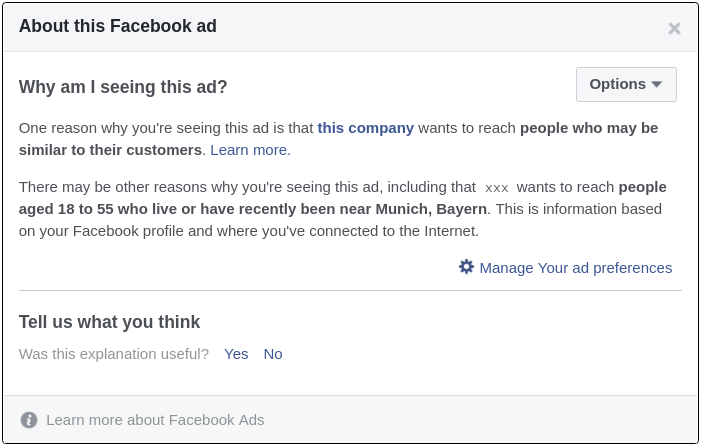
\includegraphics[scale=0.5]{img/FacebookAdExplanation2.png}
    \caption{Facebook's web-page window that provides information about what data led to users seeing Facebook's ads.}
    \label{fig:facebook_explain_book_recommendation}
\end{figure}

% -------------------------------------------------------------------------------------
\subsection*{Legitimacy}
% -------------------------------------------------------------------------------------
Legitimacy can be viewed as another step after explainability. When we provide a prediction together with sound reasoning that can be verified either by a human analyst or by another trusted system, then we can use it in more serious and sensitive deployments. One of them can be the legal domain. In it, computer systems can be used to provide unbiased and fair decisions and analyses if set up correctly. But as mentioned many times before, we need to be very careful with the data we use for training. Care needs to be taken even if we do not use an automated training solution. Most of the current systems used in the mentioned legal domain and other systems where legitimacy is required are most probably based on hand-crafted rules that can very well be subject to bias as well. One of the examples is the system COMPAS presented in Subsection \ref{subsec:02_algo_fairness.examples_of_algo_biass}.

% -------------------------------------------------------------------------------------
\subsection*{Consistency}
% -------------------------------------------------------------------------------------
For some systems, it is very important to stay consistent in outputs even with slightly different inputs. Let us assume that we are developing an illness detection algorithm that offers medical personnel some insights about their patients based on provided symptoms. The predicted recommendation should not drastically change if, for example, the temperature changes by 0.1°C. It is, therefore, closely tied to the previous properties of legitimacy and explainability. Most high-critical ML systems have to be designed with consistency in mind. Driverless cars that abruptly change direction with only a one-pixel change in the input would not induce the trust of their users.

From a different perspective, we can view fairness as a sort of consistency in the way that protected attributes of people do not affect the output. The algorithm is consistent in respect of these protected attributes.


One other meaning of consistency in regards to ML systems can be stability in the meaning of ML outputs being the same while navigating a system or an app. We can attribute it to the application's design more than the ML system itself. If a user is browsing a web page, let us say an aggregator of products on the web, they may rely on the back button while browsing the different outputs. In this setting, inconsistency and changes to the recommendation items may be harmful as they will affect the user experience while listing and using the provided information.

% -------------------------------------------------------------------------------------
\subsection*{Novelty}
% -------------------------------------------------------------------------------------
Novelty can have multiple meanings when we use it to describe RS. Firstly it can be that the item itself is a new addition to the dataset and we do not have many user-item interactions which we would use to asses and recommend the new item.

Secondly, we can say that the item is presented to the user for the first time. Sometimes, depending on the presentation of the recommended items, we have to show the recommended item repeatedly in order for it to be noticed. In that way, novelty can be viewed as a non-binary attribute, where each time we present the item to the user, it decreases the item's novelty with respect to that one user. But often, it is viewed as a binary attribute, shown or not-yet-shown.

Thirdly, by novelty, we can describe an unusual item presented to the user. Such a situation can occur either due to the RS incorrectly assuming that the user will like that item or, on purpose, introducing a new, not yet seen item so that we introduce more exploration and present items that the user will view as fresh.

And lastly, novelty is important as an exploration. RS should try to broaden and expand the model of users' preferences, which needs to be done by gathering feedback on items outside of the users' current preference model. A balance between exploration and exploitation is difficult to tune, but it can substantially increase models' performance if done correctly.

In general and contrary to the previously mentioned consistency parameter, we usually strive for novelty and exploration. If a person is picking out a movie to watch, then showing them the same selection over and over would most certainly lead to their dissatisfaction due to the limited and repeated content that the system is providing. As with all properties, novelty requirements heavily depend on the domain the system is deployed in. This property is most sought for in domains where exploration is important.




% As an example, we can imagine that in a movie recommender system a user only watched Harry Potter movies, then a RS that does not try to introduce new novel items will only recommend other Harry Potter movies which will most probably be seen as boring, repetitive and valueless.


% 3 meanings
% new item in dataset
% new item presented to user
% unusual item presented to user
% item that wasn't shown to the user that many times



Contrary to the previously mentioned consistency parameter, we sometimes strive for novelty and exploration. If a person is picking out a movie to watch, then showing them the same selection over and over would most certainly lead to their dissatisfaction due to the limited and repeated content that the system is providing. This property is most sought after in domains where exploration is important.



% -------------------------------------------------------------------------------------
\subsection*{Coverage}
% -------------------------------------------------------------------------------------
% Popsat situaci kde rs failuje v tom, ze nejake itemy jsou unreachable, nebudou pak doporuceny vsem, pripadne muzeme taky zminit to, ze popularni itemy budou vzdycky ve vyhode ktera nemusi byt uplne fair v tom, ze kdyz mas exposure tak je jednodussi dostat dalsi exposure, takovej trochu negative feedback loop. A muze se pak stavat, ze misto toho abychom doporucili item ktery je opravdu awesome pro toho uzivatele tak doporucime neco no neni tak awesome

In some ML and RS applications, there can emerge a situation where some items are never recommended. If the reason is that the item quality is bad then it can be the right system quality. In other situations, such as RS that recommends based on item properties, an undesirable behavior can occur when an item is just too different, and we do not have a reasonable 'link' to other items that would serve as a comparison for the recommendation. Then this item will be left out and never recommended.

Another coverage problem is with popular items. Popularity is sometimes a good indicator of quality, but not always. If an item is popular, then in a system that exploits popularity, it will receive more and more attention. This, in turn, further increases its popularity. In a way, we can have the same type of phenomenon as the negative feedback loop mentioned in Subsection \ref{subsubsec:02_algo_fairness.adverse_effects.nfl}. It then happens that item exposure distribution will be unnaturally skewed even more towards the popular items. This can lead to a decrease in the system's performance due to some less popular items not being recommended, even if possibly a better choice for a recommendation. In a way, popularity and unpopularity correspond to a notion of novelty where instead of considering a single user, we consider all users of the system together.


% -------------------------------------------------------------------------------------
\subsection*{Efficacy, accuracy, and precision}
% -------------------------------------------------------------------------------------
We have so far mentioned multiple other criteria. But all of them are hard to measure due to their somewhat subjective nature. Let us now present two of the most widely used exact efficacy properties: accuracy and fairness.

Accuracy (sometimes trueness) is a measure of how far away the outputs of an ML system are from the desired outputs. Precision is a measure of how unsure or dispersed the outputs are, in other words, how away are from each other. They are both measures of observation error, and the definitions differ based on the type of the outputs of the system. We can see an illustration for continuous value prediction on Figure \ref{fig:accuracy_fairness}

\begin{figure}[htbp]
    \centering
    \includesvg[width=9.5cm]{img/accuracy_and_precision.svg}
    \caption{Illustrative description of the relationship of accuracy and precision from \cite{Accuracy_precision}}
    \label{fig:accuracy_fairness}
\end{figure}

How to measure the distance of outputs to ground truth can differ based on the shape/dimensionality of the output. Usually, we use a simple metric such as Euclidean distance or simple Manhattan distance.


For categorical data, we have (binary retrieval task and multi-class classification, respectively):
\begin{equation}
    Accuracy = \dfrac{\text{TP + TN}}{\text{TP + FP + TN + FN}} = \dfrac{\text{correct classifications}}{\text{all classifications}}
\end{equation}
and precision for binary classification:
\begin{equation}
    Precision = \dfrac{\text{TP}}{\text{TP + FP}}
\end{equation}

Precision for categorical data does not have a set meaning, we can either use precision for each class separately or have one class that acts as an FP label.

Difficulties with using accuracy arise when labels are missing some or all items in the dataset. Calculating the correct denominator in categorical cases or the correct distance to the reference value can be difficult or/and impossible.

% -------------------------------------------------------------------------------------
\subsection*{Performance and scalability}
% -------------------------------------------------------------------------------------

We can design any algorithm we want, but what for will it be if we cannot then use it in the real world? Theoretical algorithms certainly have their place, but we are aiming to solve real problems of addressing fairness. Therefore another and last discussed property will be performed and, with it, the related property of scalability.

The performance of a system can be described either in a form of total computational resources needed for processing, or the whole deployment or normalized to a single user. Another possible performance property can be the length of time needed for the processing of a single request called latency. These two properties usually need to be balanced against each other. To a certain point, we can either add more computational capacity to improve - decrease latency, or remove some capacity with the possible increase in latency.

Scalability is a property of a system that it is able to handle a growing amount of work. We have to keep this property in mind while designing ML and RS systems. If, for example, we are using a comparison with other users, such as in the case of some RS algorithm, we will be growing the system requirements most probably linearly with the number of users. This can be fine in for example research applications but becomes a real concern when applied to worldwide applications used by millions of users. At these scales, we will be required to scale using not only vertical scaling (that is using more powerful computational resources), but mainly using horizontal scaling (by using many computers at once).


% TODO: Fairness is not the only property we can try to manage, what about privacy, accuracy, precision, coverage, diversity, novelty and so on. Mention them first in an overview, then separately in subsections in more detail. Try to define them mathematically.
